\bookchapter{Protobuf Serialization}\label{ch:rust8}

\section*{Explanation}
In Chapter~\ref{ch:rust7} we built a packet byte by byte. That works, but it has problems that grow with the project: every change of the layout must be made in the robot program, in the debug client, in the log reader and in the Python prototype; old log files become unreadable; and it is easy to make two sides disagree about a position or a unit. \textbf{Serialization} is the general name for turning a data structure into bytes (and back), and \textbf{Protocol Buffers} (\textbf{protobuf}) is a widely used system that solves these problems: you describe the messages \emph{once} in a small text file, and a tool generates the code for Rust, Python, C++ and many other languages. The bytes are compact, and the format can \emph{grow} without breaking older programs. The team uses protobuf for the data between robot and debug client and for the log files.

\begin{center}
\begin{tikzpicture}[>={Stealth[length=2.4mm]},bx/.style={draw,thick,rounded corners=2pt,minimum height=0.9cm,font=\footnotesize,align=center}]
 \node[bx,fill=yellow!25,minimum width=3.2cm] (pr) at (5.2,1.5) {\texttt{robot.proto}\\ (the description)};
 \node[bx,fill=orange!15,minimum width=2.6cm] (rs) at (0,-0.3) {Rust code\\ (robot, client)};
 \node[bx,fill=blue!10,minimum width=2.6cm] (py) at (5.2,-0.3) {Python code\\ (analysis)};
 \node[bx,fill=gray!15,minimum width=2.6cm] (cp) at (10.4,-0.3) {other languages};
 \draw[->,thick] (pr)--node[left,font=\scriptsize]{generate} (rs);
 \draw[->,thick] (pr)-- (py); \draw[->,thick] (pr)-- (cp);
\end{tikzpicture}
\captionof{figure}{One description, many languages: all sides use the same messages, so they cannot disagree.}
\end{center}

\section*{Formats compared}
The same message (sequence number $7$, a time stamp, and three angles), in different formats:
\begin{center}
\renewcommand{\arraystretch}{1.2}
\begin{tabular}{lrp{6.5cm}}
\textbf{format} & \textbf{bytes} & \textbf{remark}\\ \hline
JSON text & 70 & human readable, slow to parse, numbers as text\\
hand-made binary (Chapter~\ref{ch:rust7}) & 28 & smallest to decode, but nothing can be added\\
protobuf & 24 & compact, numbered fields, grows without breaking\\
\end{tabular}
\end{center}
(These sizes were measured with the messages defined below; the JSON is the compact text \verb!{"seq":7,"t_us":123456789,"imu":{"roll":0.5,...}}!.) Protobuf is not always smaller than a hand-made layout, since each field carries a one-byte tag, but it \emph{leaves out} fields that are zero or missing, and numbers such as small counters need only one or two bytes. The big advantage is not size but \textbf{evolution} and \textbf{tools}. Other formats exist (MessagePack, FlatBuffers, Cap'n Proto, the CDR of DDS, \verb!bincode! and \verb!serde! in Rust). We use protobuf because it is well supported in every language the team uses.

\section*{The \texttt{.proto} file}
%\verb!robot.proto!
\begin{verbatim}
syntax = "proto3";
package robot;

message Imu {
  float roll  = 1;     // degrees
  float pitch = 2;
  float yaw   = 3;
}

message Telemetry {
  uint32 seq   = 1;
  uint64 t_us  = 2;    // microseconds since the robot started
  Imu    imu   = 3;
  string note  = 4;
  repeated float joints = 5;   // joint angles, radians
}
\end{verbatim}
Each field has a \textbf{type}, a \textbf{name} and a \textbf{field number}. The numbers are what is sent over the network; the names are only for the programmers. Frequently used types:
\begin{center}
\renewcommand{\arraystretch}{1.2}
\begin{tabular}{ll}
\verb!int32 int64 uint32 uint64! & integers (variable length, small numbers are short)\\
\verb!sint32 sint64! & integers that are often negative\\
\verb!fixed32 fixed64 sfixed32! & integers that always take $4$ or $8$ bytes\\
\verb!float double! & floating point\\
\verb!bool!, \verb!string!, \verb!bytes! & truth value, UTF-8 text, raw bytes\\
\verb!repeated T! & a list of values of type \verb!T!\\
\verb!message! & a nested message, as \verb!Imu! above\\
\verb!enum! & a named integer value\\
\verb!oneof! & exactly one of several fields (like a Rust enum)\\
\verb!map<K, V>! & a dictionary\\
\end{tabular}
\end{center}
In proto3 a field that has its default value ($0$, empty text, \verb!false!) is \emph{not sent} and reads as the default at the other end. If you must distinguish ``$0$'' from ``not set'', declare it \verb!optional!; then the generated Rust type is \verb!Option<T>! (Chapter~\ref{ch:rust4}). Messages are also what you want for the \emph{whole protocol}: wrap all kinds in one envelope with \verb!oneof!:
\begin{verbatim}
message Packet {
  uint32 seq = 1;
  oneof payload {
    Telemetry telemetry = 2;
    Command   command   = 3;
    Log       log       = 4;
  }
}
\end{verbatim}
In Rust this becomes an \verb!enum! with one variant per case and a \verb!match! that the compiler checks for completeness, exactly the design of Chapter~\ref{ch:rust4}.

\section*{What the bytes look like}
You do not have to know the wire format to use protobuf, but looking at it removes the mystery, and it helps when you debug a packet with \verb!tcpdump! or look at a log in a hex editor. The encoding is a list of \textbf{fields}, each one a \textbf{tag} followed by a value. The tag is a number, encoded as a variable-length integer, containing the field number and the \textbf{wire type}:
\begin{center}
\verb!tag = (field_number << 3) | wire_type!
\end{center}
\begin{center}
\renewcommand{\arraystretch}{1.2}
\begin{tabular}{cp{5.6cm}p{5.2cm}}
\textbf{wire type} & \textbf{used for} & \textbf{value}\\ \hline
0 & \verb!int32 uint64 bool enum ...! & a varint\\
1 & \verb!fixed64 double! & 8 bytes, little endian\\
2 & \verb!string bytes message repeated(packed)! & a varint length, then that many bytes\\
5 & \verb!fixed32 float! & 4 bytes, little endian\\
\end{tabular}
\end{center}
A \textbf{varint} stores an integer in groups of $7$ bits, least significant group first. The highest bit of each byte says ``more bytes follow''. The number $150=10010110_2$ is split into the groups $0010110$ (low) and $0000001$ (high), and written \verb!96 01!: the first byte is $1\,0010110=0x96$ (the $1$ says ``continue''), the second $0\,0000001=0x01$.
\begin{center}
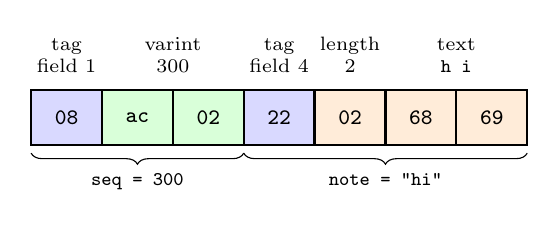
\begin{tikzpicture}[font=\scriptsize,x=0.9cm]
 \foreach \a/\t/\c in {0/08/blue!15, 1/ac/green!15, 2/02/green!15, 3/22/blue!15, 4/02/orange!15, 5/68/orange!15, 6/69/orange!15}{
   \draw[fill=\c,thick] (\a,0) rectangle (\a+1,0.7); \node[font=\ttfamily\footnotesize] at (\a+0.5,0.35) {\t};}
 \node[anchor=south,align=center] at (0.5,0.8) {tag\\ field 1};
 \node[anchor=south,align=center] at (2,0.8) {varint\\ $300$};
 \node[anchor=south,align=center] at (3.5,0.8) {tag\\ field 4};
 \node[anchor=south,align=center] at (4.5,0.8) {length\\ 2};
 \node[anchor=south,align=center] at (6,0.8) {text\\ \texttt{h i}};
 \draw[decorate,decoration={brace,mirror,amplitude=4pt}] (0,-0.1) -- (3,-0.1) node[midway,below=4pt]{\texttt{seq = 300}};
 \draw[decorate,decoration={brace,mirror,amplitude=4pt}] (3,-0.1) -- (7,-0.1) node[midway,below=4pt]{\texttt{note = "hi"}};
\end{tikzpicture}
\captionof{figure}{The bytes \texttt{08 ac 02 22 02 68 69}: field 1 (\texttt{seq}) as varint $300$ ($0xac\,0x02$: $0x2c+2\cdot128=300$), field 4 (\texttt{note}) as the two-byte text ``hi''. The tag \texttt{08} is $(1\ll3)|0$, the tag \texttt{22} is $(4\ll3)|2$.}
\end{center}
Negative numbers in an \verb!int32! are expensive (always $10$ bytes), so use \verb!sint32! when values are often negative: it applies the \textbf{zigzag} mapping $0,-1,1,-2,2,\dots\to0,1,2,3,4,\dots$, which keeps small numbers small.

To check this we wrote a small encoder and decoder by hand, without any library, in Rust. The reference bytes in the comments were produced by Python's official protobuf library from the \verb!.proto! file above (so Rust and Python were compared, not Rust with its own opinion):
%rs:wire
\begin{verbatim}
fn put_varint(out: &mut Vec<u8>, mut v: u64) {
    while v >= 0x80 {
        out.push((v as u8 & 0x7f) | 0x80);
        v >>= 7;
    }
    out.push(v as u8);
}

fn get_varint(b: &[u8]) -> Option<(u64, usize)> {
    let mut v = 0u64;
    for (i, &byte) in b.iter().enumerate().take(10) {
        v |= ((byte & 0x7f) as u64) << (7 * i);
        if byte & 0x80 == 0 { return Some((v, i + 1)); }
    }
    None                                  // too short or longer than 10 bytes
}

fn put_tag(out: &mut Vec<u8>, field: u32, wire: u8) {
    put_varint(out, ((field << 3) | wire as u32) as u64);
}
fn put_u(out: &mut Vec<u8>, field: u32, v: u64) {
    if v != 0 { put_tag(out, field, 0); put_varint(out, v); }
}
fn put_f32(out: &mut Vec<u8>, field: u32, v: f32) {
    if v != 0.0 { put_tag(out, field, 5); out.extend(v.to_le_bytes()); }
}
fn put_bytes(out: &mut Vec<u8>, field: u32, b: &[u8]) {
    if !b.is_empty() {
        put_tag(out, field, 2);
        put_varint(out, b.len() as u64);
        out.extend(b);
    }
}

fn hex(b: &[u8]) -> String {
    b.iter().map(|x| format!("{x:02x}")).collect()
}

fn imu(roll: f32, pitch: f32, yaw: f32) -> Vec<u8> {
    let mut m = Vec::new();
    put_f32(&mut m, 1, roll);
    put_f32(&mut m, 2, pitch);
    put_f32(&mut m, 3, yaw);
    m
}

fn main() {
    let mut a = Vec::new();                         // seq=7, t_us=123456789
    put_u(&mut a, 1, 7);
    put_u(&mut a, 2, 123_456_789);
    println!("{}", hex(&a));

    let mut b = a.clone();                          // ... and the nested imu
    put_bytes(&mut b, 3, &imu(0.5, -1.25, 90.0));
    println!("{} ({} bytes)", hex(&b), b.len());

    let mut c = Vec::new();                         // seq=300, note, joints
    put_u(&mut c, 1, 300);
    put_bytes(&mut c, 4, b"hi");
    let mut packed = Vec::new();                    // repeated float: packed
    for j in [0.0f32, 1.0, -1.0] { packed.extend(j.to_le_bytes()); }
    put_bytes(&mut c, 5, &packed);
    println!("{}", hex(&c));

    println!("{:?} {:?}", get_varint(&[0x96, 0x01]), get_varint(&[0x80]));
}
\end{verbatim}
prints (the first three lines are exactly what Python's \verb!SerializeToString()! gives for the same messages):
\begin{verbatim}
080710959aef3a
080710959aef3a1a0f0d0000003f150000a0bf1d0000b442 (24 bytes)
08ac02220268692a0c000000000000803f000080bf
Some((150, 2)) None
\end{verbatim}
Read the second line from the left: \verb!08 07! (field 1, value $7$), \verb!10 95 9a ef 3a! (field 2, the varint for $123\,456\,789$, five bytes), \verb!1a 0f! (field 3, a nested message of $15$ bytes) containing \verb!0d 0000003f! (field 1, float $0.5$), \verb!15 0000a0bf! (field 2, float $-1.25$) and \verb!1d 0000b442! (field 3, float $90.0$). The list of joints in the third message is \emph{packed}: one tag, a length ($12$), then the three floats. The decoder side is the mirror image and shows the mechanism that makes protobuf evolvable:
%rs:decode
\begin{verbatim}
fn get_varint(b: &[u8]) -> Option<(u64, usize)> {   // as before
    let mut v = 0u64;
    for (i, &x) in b.iter().enumerate().take(10) {
        v |= ((x & 0x7f) as u64) << (7 * i);
        if x & 0x80 == 0 { return Some((v, i + 1)); }
    }
    None
}

#[derive(Debug)]
enum Value<'a> { Varint(u64), Fixed32(u32), Bytes(&'a [u8]) }

fn fields(mut b: &[u8]) -> Result<Vec<(u32, Value<'_>)>, String> {
    let mut out = Vec::new();
    while !b.is_empty() {
        let (tag, n) = get_varint(b).ok_or("bad tag")?;
        b = &b[n..];
        let (field, wire) = ((tag >> 3) as u32, (tag & 7) as u8);
        let v = match wire {
            0 => { let (v, n) = get_varint(b).ok_or("bad varint")?;
                   b = &b[n..]; Value::Varint(v) }
            5 => { let x = b.get(..4).ok_or("short f32")?;
                   b = &b[4..];
                   Value::Fixed32(u32::from_le_bytes(x.try_into().unwrap())) }
            2 => { let (len, n) = get_varint(b).ok_or("bad length")?;
                   b = &b[n..];
                   let x = b.get(..len as usize).ok_or("short field")?;
                   b = &b[len as usize..]; Value::Bytes(x) }
            w => return Err(format!("unsupported wire type {w}")),
        };
        out.push((field, v));
    }
    Ok(out)
}

fn main() {
    // seq=7, t_us=123456789, imu {...}: a message from a NEWER sender
    let msg = [0x08, 0x07, 0x10, 0x95, 0x9a, 0xef, 0x3a, 0x1a, 0x0f,
               0x0d, 0x00, 0x00];                    // cut short on purpose
    println!("{:?}", fields(&msg));
    let ok = [0x08, 0x07, 0x10, 0x95, 0x9a, 0xef, 0x3a, 0x62, 0x01, 0x7a];
    for (f, v) in fields(&ok).unwrap() {
        match (f, v) {
            (1, Value::Varint(s)) => println!("seq = {s}"),
            (2, Value::Varint(t)) => println!("t_us = {t}"),
            (f, _) => println!("field {f}: unknown, skipped"),
        }
    }
}
\end{verbatim}
prints
\begin{verbatim}
Err("short field")
seq = 7
t_us = 123456789
field 12: unknown, skipped
\end{verbatim}
The decoder never crashes on bad input (the first message is cut off in the middle of a nested message and gives an error, Chapter~\ref{ch:rust7}), and it \emph{skips fields that it does not know}: the second message contains a field number $12$ that a newer robot program has added. The old client shows the fields it knows and ignores the rest. That is the key to evolution.
\begin{keyidea}[Rules for changing a protobuf protocol]
You may \emph{add} new fields with new numbers, and old programs will ignore them. You may \emph{remove} a field if you write \verb!reserved 7;! so the number is never reused. You must \emph{never change the number or the type} of an existing field, because old logs and old programs read the number. Rename fields freely: the name is not in the bytes. Never reuse a number: an old log would be read with the wrong meaning, silently.
\end{keyidea}

\section*{Using protobuf in Rust: the \texttt{prost} crate}
The usual Rust library is \textbf{prost}. It generates a plain Rust struct for each message at build time. The following was \emph{not run} for this book, because the computer used to write it has no access to \verb!crates.io!; the program above shows what it does inside. The version numbers are those current when this chapter was written (prost $0.14$); check \verb!crates.io!, because the API of crates changes between releases.
\begin{verbatim}
# Cargo.toml
[dependencies]
prost = "0.14"
[build-dependencies]
prost-build = "0.14"
\end{verbatim}
\begin{verbatim}
// build.rs  (runs before the compilation of the crate)
fn main() -> std::io::Result<()> {
    prost_build::compile_protos(&["proto/robot.proto"], &["proto/"])?;
    Ok(())
}
\end{verbatim}
\begin{verbatim}
// src/lib.rs
pub mod robot {
    include!(concat!(env!("OUT_DIR"), "/robot.rs"));   // generated code
}

use prost::Message;
use robot::{Imu, Telemetry};

fn demo() -> Result<(), prost::DecodeError> {
    let t = Telemetry {
        seq: 7,
        t_us: 123_456_789,
        imu: Some(Imu { roll: 0.5, pitch: -1.25, yaw: 90.0 }),
        note: String::new(),
        joints: vec![],
    };
    let bytes: Vec<u8> = t.encode_to_vec();        // 24 bytes
    let back = Telemetry::decode(bytes.as_slice())?;
    assert_eq!(t, back);
    Ok(())
}
\end{verbatim}
Points to know: (1) \verb!prost-build! needs the program \verb!protoc! (the protobuf compiler) on the machine; on Ubuntu \verb!sudo apt install protobuf-compiler!, or use a crate that brings its own copy. (2) A nested message becomes an \verb!Option<Imu>!, because ``not sent'' is possible; scalars are plain values; \verb!repeated! becomes \verb!Vec!; a \verb!oneof! becomes an \verb!enum! (in a submodule). (3) \verb!decode! returns a \verb!Result!, so a bad packet is an error and not a crash (Chapter~\ref{ch:rust5}). (4) Generated code lives in the \verb!target! folder and is not committed; the \verb!.proto! file is. (5) For Python: \verb!protoc --python_out=. robot.proto! creates \verb!robot_pb2.py!, and \verb!robot_pb2.Telemetry(seq=7).SerializeToString()! gives the bytes (this is how our prototype and the analysis scripts read the same logs). (6) Put the \verb!.proto! file and the generated code into the \emph{shared library crate} of the workspace of Chapter~\ref{ch:rust5}, used by robot, client and the log tools.

\section*{Datagrams and log files}
One UDP datagram contains one message; the boundary is given by the network, no framing is needed. A \emph{file} or a TCP stream has no boundaries, so each message is preceded by its length as a varint, the \textbf{length-delimited} format (\verb!encode_length_delimited! in prost). A log is then a sequence of ``length, message, length, message, \dots''. A reader can \emph{skip} through the file without decoding, and a robot that crashed in the middle of a write leaves only the last record damaged. The following program writes records with a time stamp and the nested bytes from above, cuts the file in the middle of the last record, and reads back everything that is intact:
%rs:log
\begin{verbatim}
use std::fs;

fn put_varint(out: &mut Vec<u8>, mut v: u64) {
    while v >= 0x80 { out.push((v as u8 & 0x7f) | 0x80); v >>= 7; }
    out.push(v as u8);
}
fn get_varint(b: &[u8]) -> Option<(u64, usize)> {
    let mut v = 0u64;
    for (i, &x) in b.iter().enumerate().take(10) {
        v |= ((x & 0x7f) as u64) << (7 * i);
        if x & 0x80 == 0 { return Some((v, i + 1)); }
    }
    None
}

fn read_records(data: &[u8]) -> Vec<&[u8]> {
    let (mut recs, mut pos) = (Vec::new(), 0);
    while let Some((len, n)) = get_varint(&data[pos..]) {
        let (start, end) = (pos + n, pos + n + len as usize);
        if end > data.len() { break; }            // incomplete last record
        recs.push(&data[start..end]);
        pos = end;
    }
    recs
}

fn main() -> std::io::Result<()> {
    let mut file = Vec::new();
    for seq in 1..=1000u64 {
        let rec = [&[0x08][..], &{ let mut v = Vec::new();
                                    put_varint(&mut v, seq); v }].concat();
        put_varint(&mut file, rec.len() as u64);
        file.extend(rec);
    }
    let path = std::env::temp_dir().join("demo.log");
    fs::write(&path, &file)?;
    println!("file size {} bytes", file.len());

    let mut data = fs::read(&path)?;
    println!("intact records: {}", read_records(&data).len());
    data.truncate(data.len() - 1);          // crash in the last record
    println!("after crash:    {}", read_records(&data).len());
    fs::remove_file(path)?;
    Ok(())
}
\end{verbatim}
prints \verb!file size 3873 bytes!, \verb!intact records: 1000! and \verb!after crash:    999!. Each of the $1000$ messages costs $3$ to $4$ bytes (length, tag, a one- or two-byte number), $3.9$ bytes on average ($3873/1000$). Protobuf logs compress very well (\verb!zstd! or \verb!gzip!), and one can \emph{stream} them: a program that processes a $10$\,GB log needs no more memory than one record.

\begin{aibox}[One source of truth]
Put the \texttt{.proto} file in the repository, review changes to it like code, and generate the code for every language in the build. Add a test that encodes a message in Rust and decodes it in Python (or the other way round) with a fixed example file, so that a change on one side is caught at once. The most expensive protocol bugs are the quiet ones, where both sides run happily but disagree about a unit or a field.
\end{aibox}

\section*{Practice problems}
\begin{enumerate}[label=\textbf{\thechapter.\arabic*}]
  \item Compute the tag byte for field number $3$ with wire type $2$, and for field number $15$ with wire type $5$. Why are field numbers $1$ to $15$ valuable?
  \item Encode the varint for $300$ by hand (the bit groups, the continuation bits). Check with the example of the figure. How many bytes need the numbers $127$, $128$, $16383$ and $16384$?
  \item Decode the bytes \verb!08 96 01 12 03 61 62 63! by hand: which fields do they contain and with which values?
  \item Why does a message with all fields at their default values take $0$ bytes? What is the consequence for the receiver if the sender \emph{really} meant ``$0$'' and the field was declared \verb!optional! or not?
  \item Compute the zigzag value of $-3$, $3$, $-100$ (formula $(n\ll1)\oplus(n\gg31)$ for $32$-bit numbers) and the inverse of $7$ and of $8$. Why does it help for small negative numbers?
  \item Write a \verb!.proto! description for a message \verb!JointState! with the joint name (text), the position, the velocity and the temperature (floats), and a message \verb!RobotState! with a time stamp and a list of \verb!JointState!. Which field numbers do you give to the fields that are sent at the highest rate?
  \item The robot program sends version $2$ of \verb!Telemetry!, which has a new field \verb!battery_v = 6!. The debug client still has version $1$. What does the client do with the new field? What would go wrong if somebody \emph{changed} the type of field $2$ from \verb!uint64! to \verb!double!?
  \item Design the envelope \verb!Packet! with a \verb!oneof! for three kinds of messages (telemetry, command, log text). Write the Rust \verb!match! (as pseudo code) that handles all of them. What happens in the Rust code when you add a fourth kind in the \verb!.proto!?
  \item Why would you not use protobuf (or any binary format) for a configuration file that people edit, and what would you use? Why is protobuf a good choice for log files?
  \item[\textbf{\thechapter.10}$\star$] Extend the hand-written encoder of this chapter by a function \verb!put_sint32! with zigzag, and a decoder function that reads a \verb!Telemetry! (with the fields seq, t\_us and the three floats of the nested \verb!Imu!) from bytes, ignoring unknown fields. Test with the bytes of the second line of the chapter and with the same bytes followed by an unknown field.
\end{enumerate}
